\documentclass{article}
\usepackage[T1]{fontenc}
\usepackage{lmodern}
\usepackage{graphicx}
\usepackage{amsmath,amssymb}
\usepackage[a4paper,margin=2cm]{geometry}
\usepackage[absolute,overlay]{textpos}
\setlength{\TPHorizModule}{1mm}
\setlength{\TPVertModule}{1mm}
\usepackage[indonesian]{babel}
\usepackage{hyperref}
\setlength{\emergencystretch}{2em}
% unit: Halaman 49

\begin{document}

% === Halaman 49 (llm) ===

\vspace{250.97mm}

\begin{center}
\Large Man-in-the-middle-attack
\end{center}

\vspace{10mm}

% deskripsi: Diagram ilustrasi serangan Man-in-the-middle yang menunjukkan seorang pengguna (User) dan situs web (Website) yang koneksi aslinya terputus dan dialihkan melalui penyerang (Attacker/Man in the middle) melalui koneksi baru.
% bbox normalisasi: [0.2010, 0.1110, 0.7960, 0.9560]
\begin{textblock*}{124.95mm}(42.21mm,32.97mm)
\noindent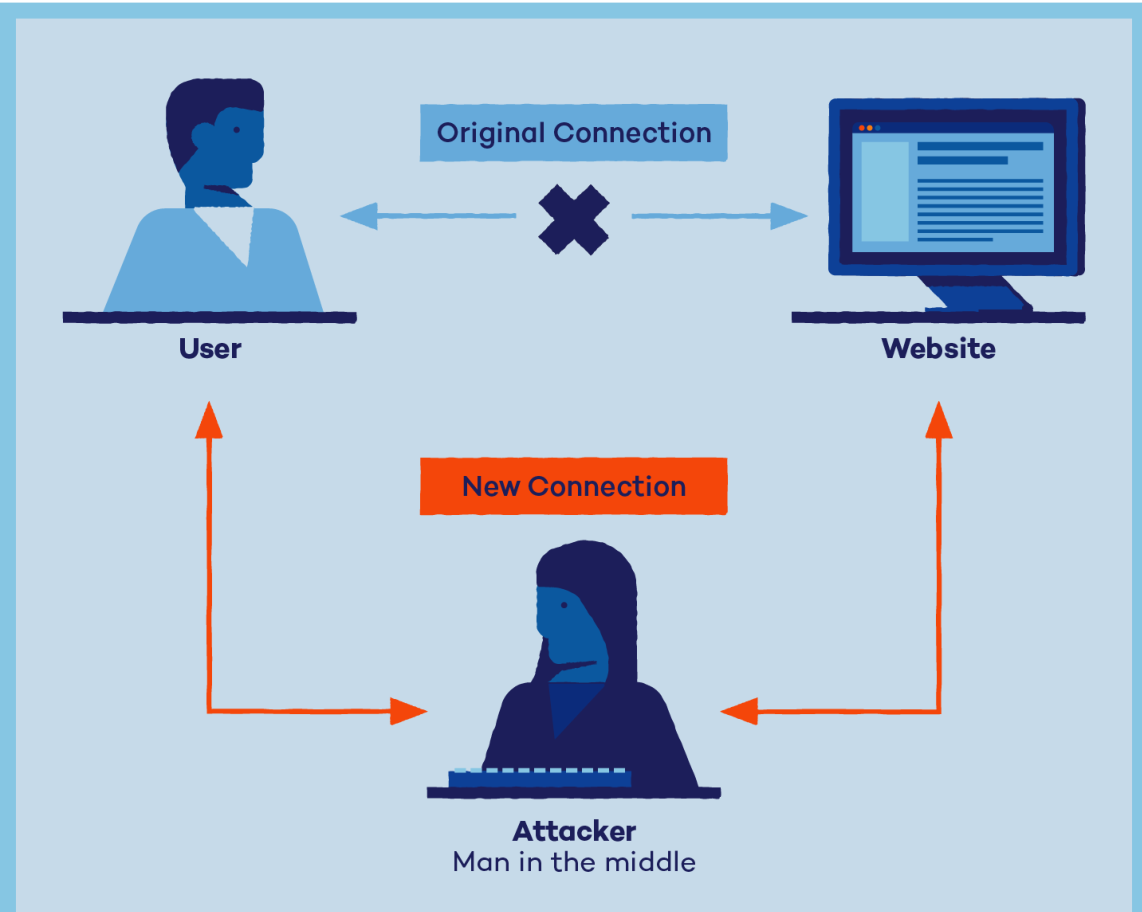
\includegraphics[width=124.95mm,height=250.97mm]{../../images/llm/page_049_img_01.png}%
\end{textblock*}

\end{document}
